\section{\textbf{Testes e análises do \textit{software}}}
\label{testes_do_software}
O \textit{software} criado no decorrer deste projeto é um simples exemplo do uso de técnicas de visão computacional aplicadas no reconhecimento de jogadores de futebol americano. Para validar a efetividade do sistema, foram criados vários cenários para testar o desempenho do algoritmo. Sendo assim, as figuras a seguir representam os testes feitos com o sistema desenvolvido, bem como uma avaliação do seu desempenho.

Inicialmente, o algoritmo foi testado em um cenário com imagens estáticas, como pode ser visto na \autoref{fig_comparativo_img} e \autoref{fig_rec_numero}, no qual ele analisa esta imagem, extraindo todos os seus padrões de características. Em seguida, ele realiza uma busca por similaridade na mesma imagem onde pode-se notar, com maior evidência na  \autoref{fig_comparativo_img} que, mesmo ele cometendo alguns erros na parte de extração de características e aprendizado de máquina, a etapa de aperfeiçoamento entende os padrões e realiza um balanceamento de quais característica são interessantes para serem levadas em consideração na hora de montar um modelo de busca. As características de menor interesse são dispensadas para reduzir a probabilidade do algoritmo cometer erros.

\begin{figure}[ht]
	\caption{\label{fig_rec_numero}\textbf{TESTE 02:} A imagem (A) representa os pontos de interesse encontrados nos números das camisas dos jogadores. A imagem (B) a sua identificação após o aperfeiçoamento.}
	\begin{center}
		\resizebox{1.0\linewidth}{!}{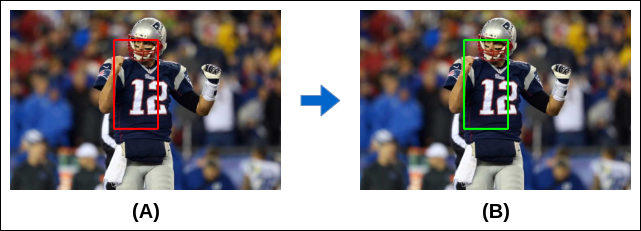
\includegraphics{6-Desenvolvimento-Projeto/imagens-desenvolvimento/representacao_numero.png}}
	\end{center}
	\centering \legend{Fonte: Elaborada pelos autores.}
\end{figure}

Como pode ser visto na \autoref{fig_rec_numero}, não existe nenhuma diferença entre utilizar o \textit{haar cascade} para realizar o reconhecimento, e a utilização de técnicas de aperfeiçoamento das características. Sendo assim, deve ser levado em consideração que, não é necessário realizar várias técnicas para resolver todo tipo de problema, pois cada análise feita pelo algoritmo utiliza altos recursos de processamento de máquina. Portanto, no caso da \autoref{fig_rec_numero} em específico, os recursos computacionais foram utilizados erroneamente.

Em seguida, o algoritmo foi colocado em um cenário de análise de vídeo de uma partida de futebol americano. Nas etapas a seguir, o algoritmo utiliza o modelo de busca já treinado para identificar um jogador de futebol americano dentro de campo.

Vale ressaltar que o algoritmo esta padronizado para identificar apenas um jogador dentro de campo.

Essas decisão foi tomada para resolver problemas de ofuscamento\footnote{Ofuscamento é a variação luminosa causada pela presença de uma ou mais fontes de luz localizada no campo visual, ocasionando uma perca visual do ambiente ou objeto \cite{LACAVA1999}.} no campo de visão do algoritmo como, por exemplo, quando um jogador passar na frente de outro jogador, situação que acontece a todo momento durante uma partida de futebol americano.

A \autoref{fig_rep_jogador_em_campo} foi retirada de um vídeo de uma partida de futebol americano. O algoritmo analisou \textit{frame} a \textit{frame} do vídeo para realizar a busca por similaridade seguindo o modelo de busca já treinado. Com base nessas informações, pode-se notar que o \textit{software} realizou uma leitura dos jogadores de futebol americano e identificou o jogador que mais se aproxima das características contidas no modelo de busca.

\begin{figure}[ht]
	\caption{\label{fig_rep_jogador_em_campo}\textbf{TESTE 03:} Identificação de um jogador em uma partida de futebol americano.}
	\begin{center}
		\resizebox{.9\linewidth}{!}{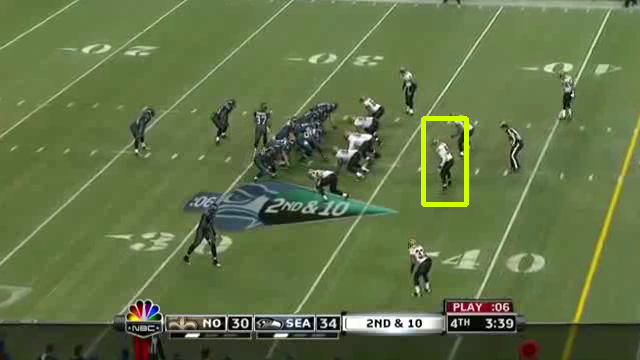
\includegraphics{6-Desenvolvimento-Projeto/imagens_teste/identificacao_jogador_em_campo_2.png}}
	\end{center}
	\centering \legend{Fonte: Elaborada pelos autores.}
\end{figure}

% Outro fator que pode ser observado na \autoref{fig_rep_jogador_em_campo} é que o algoritmo identificou somente um jogador na cena analisada. Isso ocorre porque o comportamento seguido pelo \textit{software} é de analisar o jogador e compará-lo com os padrões de características do modelo de busca, analisando também a sua fisionomia. Sendo assim, os outros jogadores podem ter atendido algum ponto de característica contido dentro do modelo de busca, porém, aquele jogador identificado é o que mais se assemelha ao modelo e por isso ele foi identificado na cena.

Já a \autoref{fig_rep_jogador_mais_evidente} mostra a identificação do jogador mais evidente no ponto de vista do algoritmo. Como pode ser visto, no meio de uma jogada de futebol americano, o jogador que mais se encaixou nos padrões de características do modelo de busca foi identificado.

\clearpage

\begin{figure}[ht]
	\caption{\label{fig_rep_jogador_mais_evidente}\textbf{TESTE 04:} Identificação do jogador mais evidente.}
	\begin{center}
		\resizebox{.7\linewidth}{!}{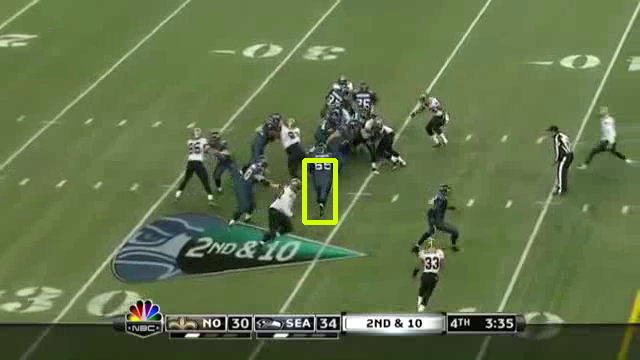
\includegraphics{6-Desenvolvimento-Projeto/imagens_teste/jogador_mais_evidente.png}}
	\end{center}
	\centering \legend{Fonte: Elaborada pelos autores.}
\end{figure}

Da mesma forma, a \autoref{fig_rep_jogador_em_movimento} representa a identificação de um jogador em movimento. Ao testar o \textit{software} nesse cenário, ele consegue, por um breve período, seguir o jogador analisado na sua corrida. Vale ressaltar que o algoritmo atual não é capaz de seguir o jogador dentro de campo durante toda a partida. Mas, com o aprimoramento da ferramenta e também do modelo de busca, esse tipo de situação pode ser feita com mais eficiência.

%\clearpage

\begin{figure}[ht]
	\caption{\label{fig_rep_jogador_em_movimento}\textbf{TESTE 05:} Identificação de um jogador em movimento dentro de campo.}
	\begin{center}
		\resizebox{.7\linewidth}{!}{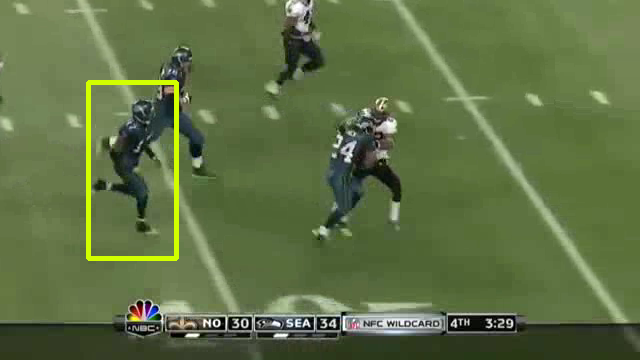
\includegraphics{6-Desenvolvimento-Projeto/imagens_teste/jogador_em_movimento.png}}
	\end{center}
	\centering \legend{Fonte: Elaborada pelos autores.}
\end{figure}

A \autoref{fig_rep_jogador_em_jogada} representa um jogador em uma velocidade mais alta do que o da \autoref{fig_rep_jogador_em_movimento}. Isso ocorreu devido a um lance que exigiu maior condicionamento físico do jogador de futebol americano. Mesmo nesse cenário, o algoritmo também foi capaz de identificar e perseguir o jogador dentro de campo por um intervalo de tempo. No entanto, o algoritmo teve um pouco mais de dificuldade para capturar todos os movimentos e realizar a identificação do  jogador devido o seu excesso de velocidade, não sendo possível persegui-lo durante um bom tempo ou até mesmo quando entra em contato com o seu adversário.

%\clearpage

\begin{figure}[ht]
	\caption{\label{fig_rep_jogador_em_jogada}\textbf{TESTE 06:} Identificação de um jogador em movimento para disputar uma jogada.}
	\begin{center}
		\resizebox{.7\linewidth}{!}{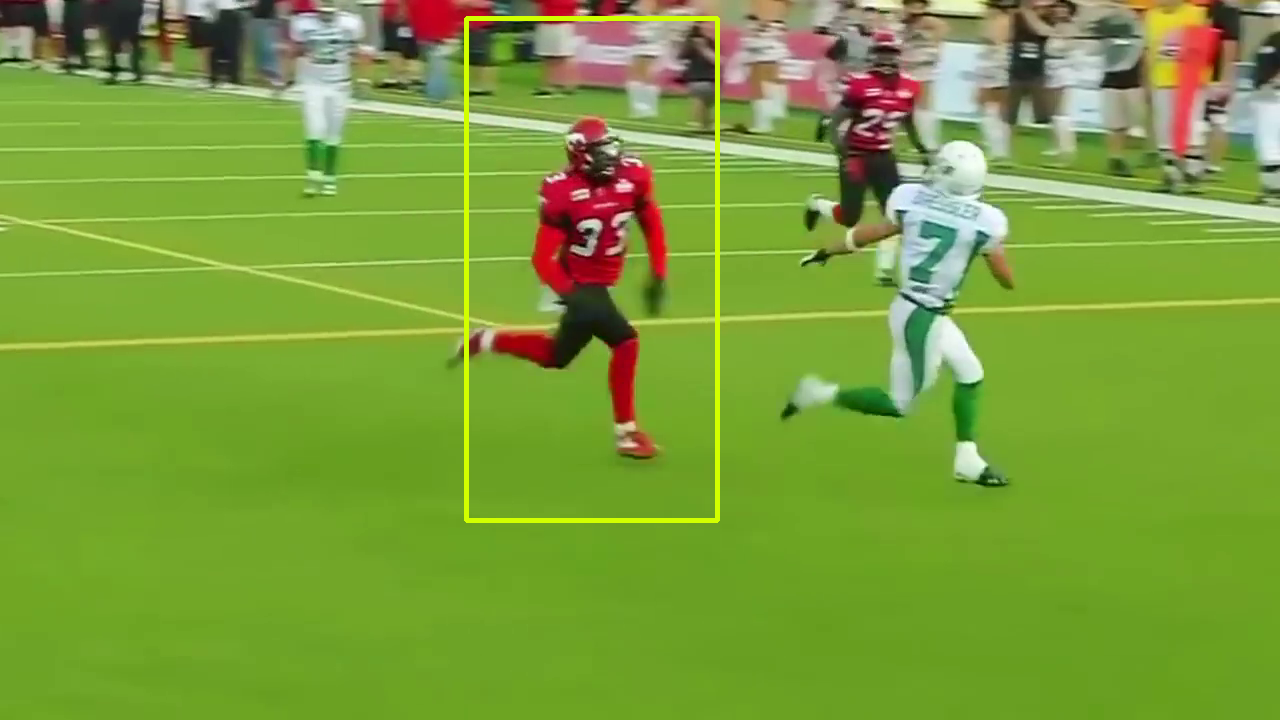
\includegraphics{6-Desenvolvimento-Projeto/imagens_teste/identificacao_jogadores_fa3.png}}
	\end{center}
	\centering \legend{Fonte: Elaborada pelos autores.}
\end{figure}

A \autoref{fig_rep_jogador_em_movimento_1} e \autoref{fig_rep_jogador_em_movimento_2} mostra como foi a tentativa do algoritmo de seguir um jogador em movimento para disputar uma jogada dentro de campo.

\begin{figure}[ht]
	\caption{\label{fig_rep_jogador_em_movimento_1}\textbf{TESTE 07:} Tentativa de seguir os movimentos de um jogador dentro de campo.}
	\begin{center}
		\resizebox{.8\linewidth}{!}{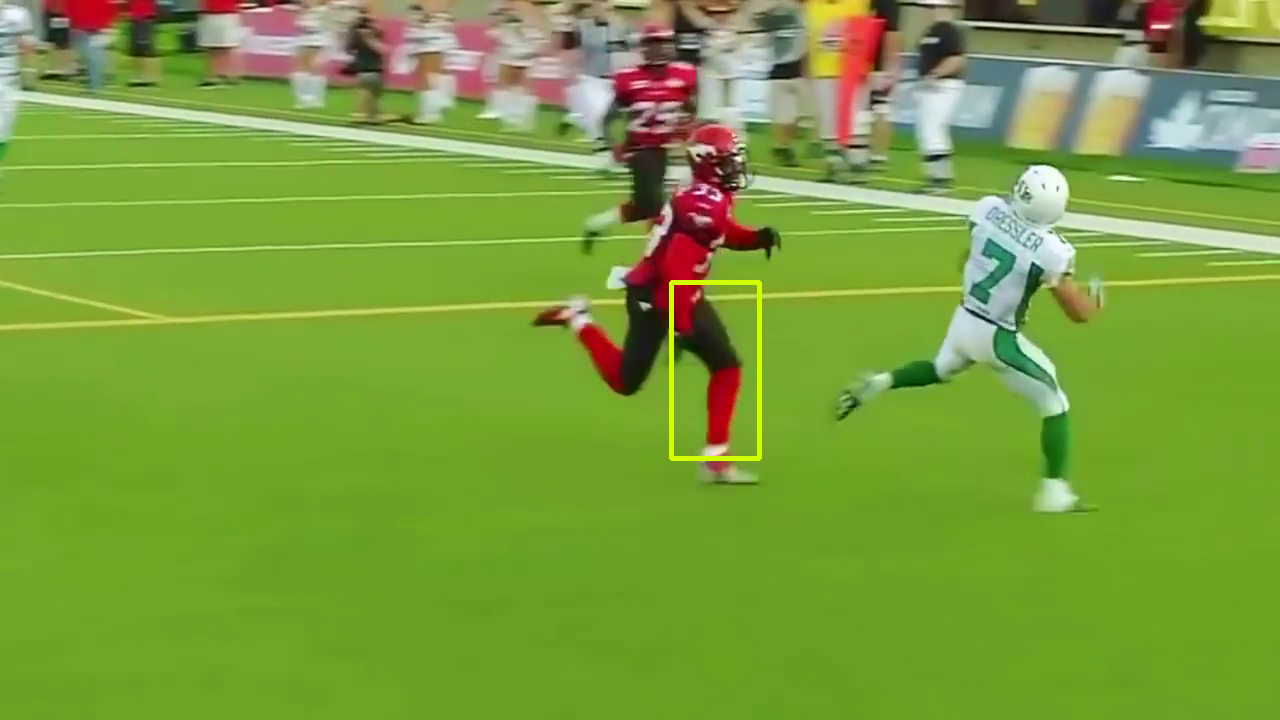
\includegraphics{6-Desenvolvimento-Projeto/imagens_teste/jogador_dentro_de_campo_1.png}}
	\end{center}
	\centering \legend{Fonte: Elaborada pelos autores.}
\end{figure}

%\clearpage

\begin{figure}[ht]
	\caption{\label{fig_rep_jogador_em_movimento_2}\textbf{TESTE 08:} Identificação do jogador de futebol americano após o movimento de corrida.}
	\begin{center}
		\resizebox{1\linewidth}{!}{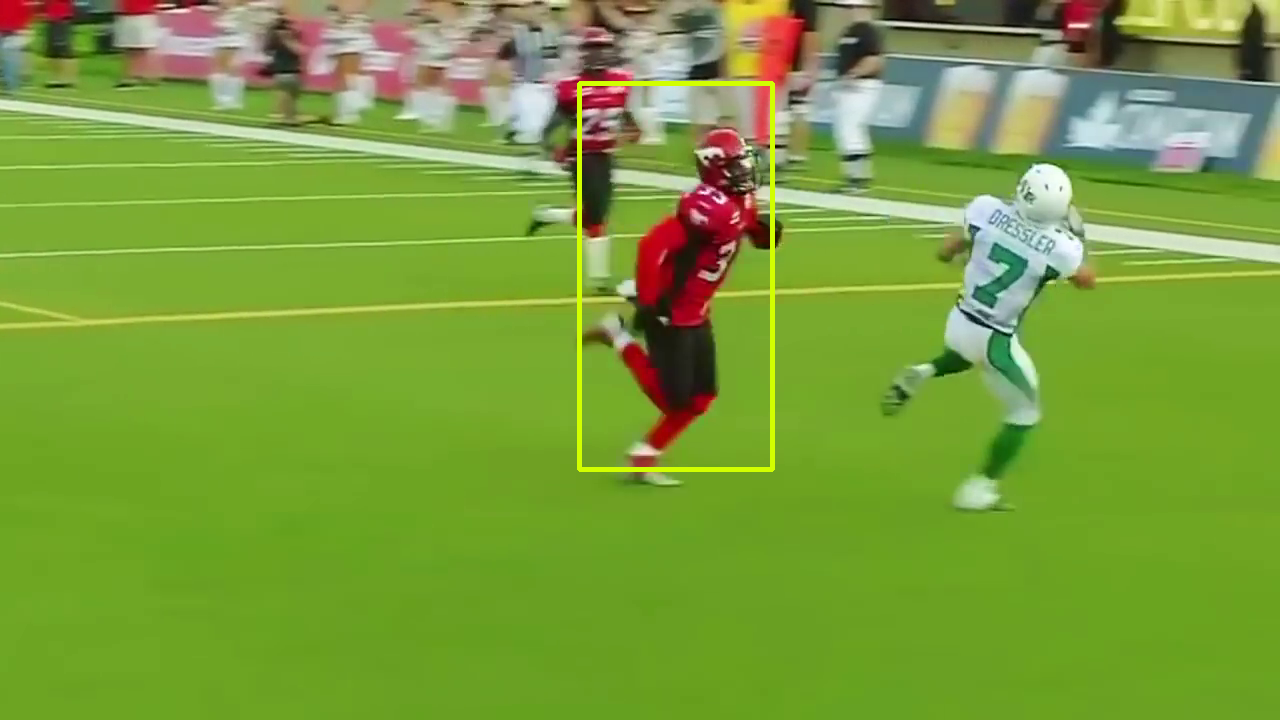
\includegraphics{6-Desenvolvimento-Projeto/imagens_teste/jogador_dentro_de_campo_9.png}}
	\end{center}
	\centering \legend{Fonte: Elaborada pelos autores.}
\end{figure}

Após a análise do \textit{frame} do vídeo representado pela \autoref{fig_rep_jogador_em_movimento_1}, no qual ele captura um movimento do jogador de futebol americano, foi realizada a mesma análise utilizando o algoritmo que analisa imagens estáticas. A \autoref{fig_rep_erro} mostra que, dependendo da situação de movimento do jogador, o algoritmo não o reconhece, e sim reconhece o seu movimento. Isso ocorre porque a maioria das imagens que foram utilizadas para treinar o algoritmo continha jogadores de futebol americano em suas devidas situações dentro de campo, ou seja, os jogadores estavam correndo, em ataque, em disputa de bola e em várias outras situações de jogo. Sendo assim, os movimentos dos jogadores de futebol americano dentro de cambo também é um fator de análise do algoritmo e, consequentemente, é algo que pode interferir na identificação do mesmo.

\clearpage

\begin{figure}[ht]
	\caption{\label{fig_rep_erro}\textbf{TESTE 09:} Identificação do movimento de um jogador de futebol americano.}
	\begin{center}
		\resizebox{.6\linewidth}{!}{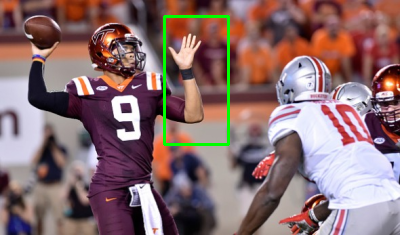
\includegraphics{6-Desenvolvimento-Projeto/imagens_teste/jogador_erro_1.png}}
	\end{center}
	\centering \legend{Fonte: Elaborada pelos autores.}
\end{figure}

A \autoref{fig_rep_erro} é outra representação onde o aprendizado de máquina não teve nenhum impacto de melhoria na identificação do conteúdo da imagem. O algoritmo continua identificando apenas um movimento do jogador, ou seja, permaneceu no erro.

A \autoref{fig_rep_dois_jogadores} representa basicamente o desempenho do algoritmo ao analisar o \textit{frame} do vídeo e identificar mais de um jogador de futebol americano dentro de campo. Como pode ser visto, o algoritmo conseguiu reconhecer dois jogadores dentro do \textit{frame} do vídeo, no entanto ele ainda não conseguiu identificar o restante.

\begin{figure}[ht]
	\caption{\label{fig_rep_dois_jogadores}\textbf{TESTE 10:} Identificação de dois jogadores de futebol americano dentro de campo.}
	\begin{center}
		\resizebox{.8\linewidth}{!}{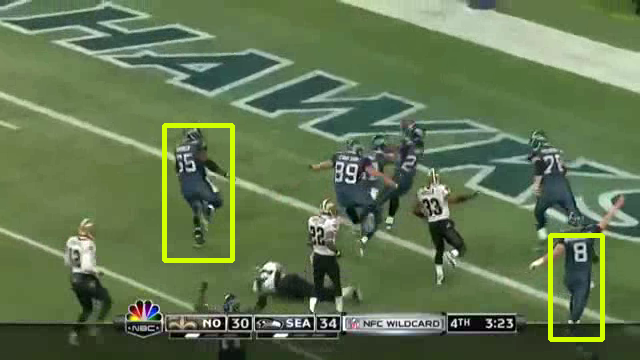
\includegraphics{6-Desenvolvimento-Projeto/imagens_teste/dois_jogadores_detectados.png}}
	\end{center}
	\centering \legend{Fonte: Elaborada pelos autores.}
\end{figure}

Já na \autoref{fig_rep_acessorios} podemos notar que o algoritmo não detectou nenhum jogador de futebol americano no \textit{frame} do vídeo. No entanto, como pode ser visto, o algoritmo conseguiu identificar alguns detalhes no uniforme dos jogadores. Isso ocorreu porque a variação dos tons de \textit{pixels} naquela região atendeu aos padrões de características extraídas das imagens de treino que foram utilizadas para gerar o modelo de busca. Dessa forma, o algoritmo entendeu que, nesse \textit{frame} em específico, os pontos de maior interesse que possuem semelhança com o modelo de busca são os identificados na imagem. No entanto, detectar esses detalhes ainda é um erro, pois isso não significa que existe um jogador de futebol americano em campo.

\begin{figure}[ht]
	\caption{\label{fig_rep_acessorios}\textbf{TESTE 11:} Identificação dos detalhes do uniforme de um jogador de futebol americano.}
	\begin{center}
		\resizebox{.9\linewidth}{!}{\includegraphics{6-Desenvolvimento-Projeto/imagens_teste/identificacao_jogadores_fa5.png}}
	\end{center}
	\centering \legend{Fonte: Elaborada pelos autores.}
\end{figure}

Outro fator muito interessante a ser analisado é a identificação feita pelo algoritmo na \autoref{fig_rep_arbitro}. Como pode ser visto, o sistema identificou o árbitro dentro de campo, e não  um dos jogadores de futebol americano. Essa situação foi bastante inusitada, pois não foi alterado nenhum parâmetro de busca e o modelo de busca também não foi alterado. Sendo assim, com base na \autoref{fig_rep_acessorios} e \autoref{fig_rep_arbitro}, pode-se concluir que a diferença de tonalidade dos uniformes também é um parâmetro que o algoritmo leva em consideração para realizar o processamento de imagem.

\clearpage

\begin{figure}[ht]
	\caption{\label{fig_rep_arbitro}\textbf{TESTE 12:} Reconhecimento do árbitro dentro de campo.}
	\begin{center}
		\resizebox{.7\linewidth}{!}{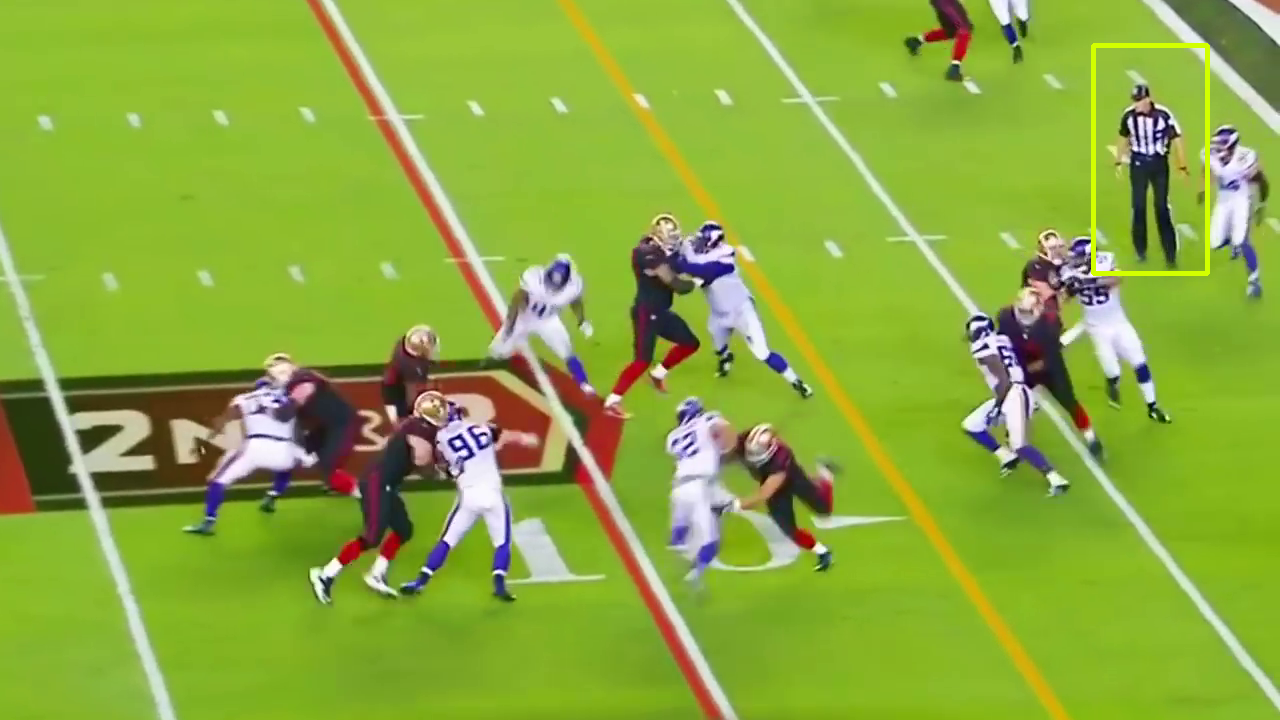
\includegraphics{6-Desenvolvimento-Projeto/imagens_teste/identificacao_arbitro.png}}
	\end{center}
	\centering \legend{Fonte: Elaborada pelos autores.}
\end{figure}

A \autoref{fig_processamento_maquina}  representa o consumo de \textit{hardware} quando o algoritmo é executado para realizar a análise de um vídeo. Como pode ser visto na parte superior da imagem, todos os recursos do processador da máquina estão sendo utilizados com grande capacidade. Sendo assim, o \textit{software} requer muito poder de processamento da máquina, consumindo grande parte dos seus recursos.  Vale lembrar que este teste foi bem simples, utilizando apenas o monitorador de processos do sistema, e mostra superficialmente os recursos necessários para a execução do algoritmo. Na \autoref{novos_estudos} foi sugerido um estudo mais avançado sobre esse consumo de \textit{hardware}.

\begin{figure}[ht]
	\caption{\label{fig_processamento_maquina}\textbf{TESTE 13:} Representação do processamento da máquina.}
	\begin{center}
		\resizebox{.7\linewidth}{!}{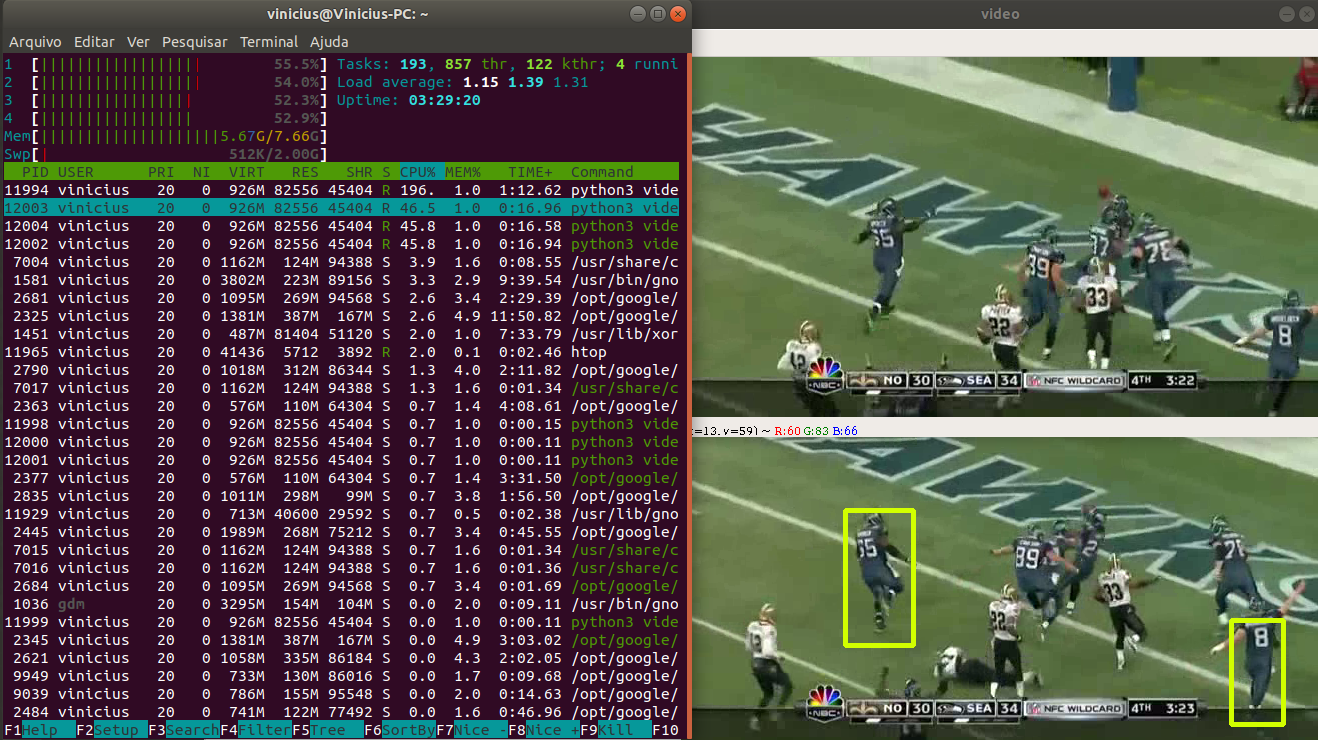
\includegraphics{6-Desenvolvimento-Projeto/imagens_teste/processamento-da-maquina1.png}}
	\end{center}
	\centering \legend{Fonte: Elaborada pelos autores.}
\end{figure}

Para resumir os resultados obtidos nos testes e análise do \textit{software}, foi feito uma tabela (\autoref{resultado_de_testes}) que tem por finalidade representar quais foram os ambientes de testes que o algoritmo mais se destacou.

\begin{table}[h]
\centering
\caption{Resumo dos resultados dos testes}
\label{resultado_de_testes}
\begin{tabular}{l|l} 
\hline
\hline
\multicolumn{1}{l|}{\textbf{Ambiente de Teste}} & \multicolumn{1}{l}{\textbf{Resultado}}  \\ 
\hline
\centering
Teste 1 - \autoref{fig_comparativo_img} & Acertou parcialmente\\
Teste 2 - \autoref{fig_rec_numero} & Acertou\\
Teste 3 - \autoref{fig_rep_jogador_em_campo} & Acertou\\
Teste 4 - \autoref{fig_rep_jogador_mais_evidente} & Acertou\\
Teste 5 - \autoref{fig_rep_jogador_em_movimento} & Acertou\\
Teste 6 - \autoref{fig_rep_jogador_em_jogada} & Acertou\\
Teste 7 - \autoref{fig_rep_jogador_em_movimento_1} & Errou\\
Teste 8 - \autoref{fig_rep_jogador_em_movimento_2} & Acertou\\
Teste 9 - \autoref{fig_rep_erro} & Errou\\
Teste 10 - \autoref{fig_rep_dois_jogadores} & Superou as expectativas\\
Teste 11 - \autoref{fig_rep_acessorios} & Errou\\
Teste 12 - \autoref{fig_rep_arbitro} & Errou\\
Teste 13 - \autoref{fig_processamento_maquina} & Desempenho da máquina\\
\hline
\hline
\end{tabular}
\centering \legend{Fonte: Elaborada pelos autores.}
\end{table}